\documentclass[class=report, crop=false, 12pt,a4paper]{standalone}
\usepackage{enumitem}
\usepackage{multicol}
\usepackage{graphicx}
\usepackage{float}
\usepackage{amsmath}
\usepackage{amssymb}
\usepackage{mathtools}
\usepackage{siunitx}
\usepackage{commath}
\usepackage{array}
\usepackage{natbib}
\usepackage[a4paper,width=150mm,top=25mm,bottom=25mm]{geometry}
\setlength{\parindent}{0pt}
\begin{document}
\begin{center}
  27/11/2020
\end{center}
\section{Plastic Hinges}
So far we have considered the case of pure bending: predicted propagation of plastic region occurs at all sections in same way. However, pure bending rarely occurs. Distribution of bending moment is commonly variable along beam length. \\\\
In this case, the section with highest bending moment would reach fully plastic state first. The fully plastic section can not react to further increase of moment: \textbf{it loses its capability of reacting to rotations and its curvature can increase indefinitely}. The section behaves like a hinge and is called \textbf{PLASTIC HINGE}.
\begin{figure}[H]
  \centering
  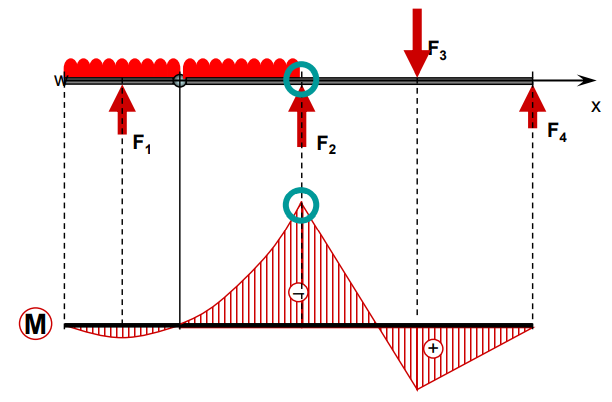
\includegraphics[width = 0.6 \textwidth]{../img/beam21.PNG}
\end{figure}
A plastic hinge is defined as a hinge which can undergo rotation when the bending moment reaches the plastic moment $M_P$.
\begin{itemize}
  \item for $M<M_P \longrightarrow$ No Rotation
  \item for $M=M_P \longrightarrow$ Rotation
  \begin{itemize}
    \item $M_P$ is the limiting value for the bending moment
  \end{itemize}
\end{itemize}
The effect of the plastic hinge is equivalent to introducing in the section an additional pin joint and a concentrated bending moment equal to $M_P$.
\subsubsection{\large Simply Supported Beam with Central Load}
\begin{figure}[H]
  \centering
  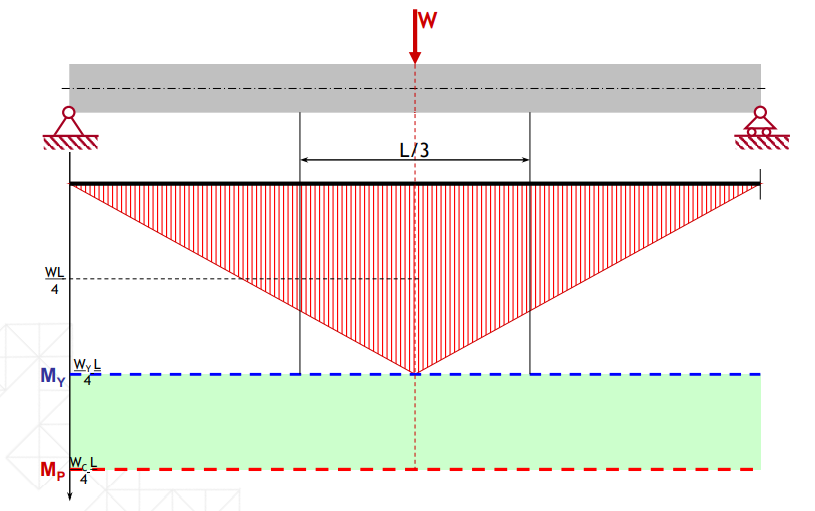
\includegraphics[width = 0.9 \textwidth]{../img/beam22.PNG}
  \caption{As W increases the bending moment raise until the yielding moment is reached at midspan. Yielding starts at midspan, at the top and bottom edges of the section, and spreads inwards to the NA and at either sides.}
\end{figure}
\begin{figure}[H]
  \centering
  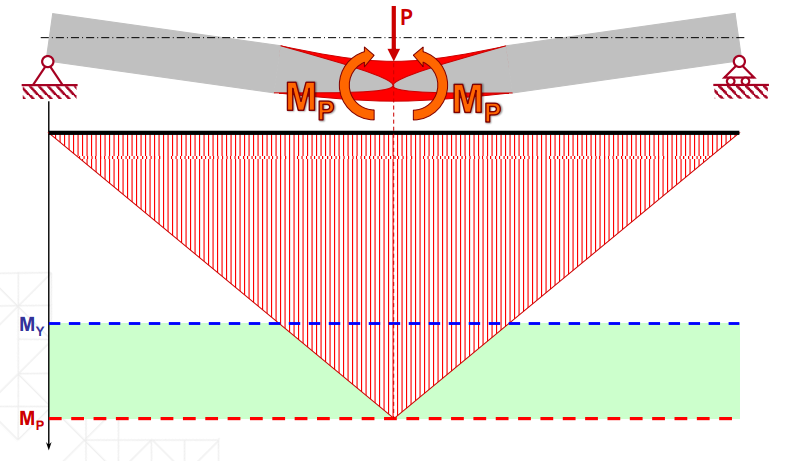
\includegraphics[width = 0.9 \textwidth]{../img/beam23.PNG}
  \caption{By the time plastic hinge forms at the midspan, yielding is quite widespread in the beam.}
\end{figure}
\begin{figure}[H]
  \centering
  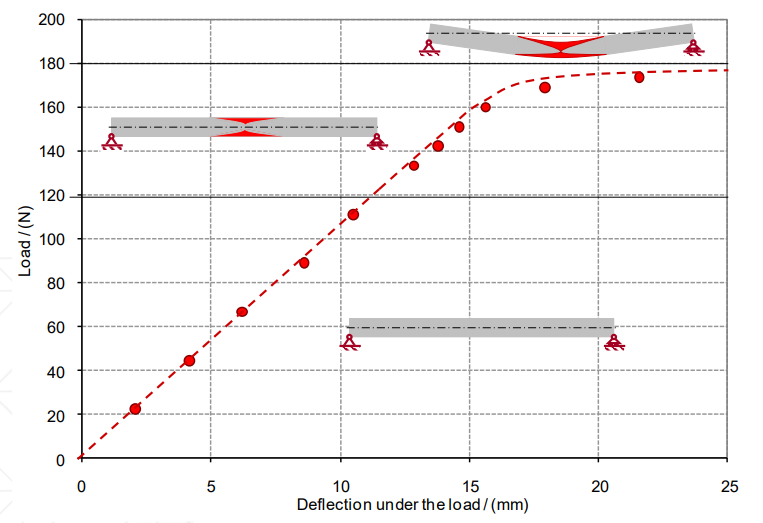
\includegraphics[width = 0.9 \textwidth]{../img/graph7.PNG}
  \caption{Experimental Load-Deflection Characteristic}
\end{figure}
\subsubsection{\large Simply Supported Beam with Uniform Load}
\begin{figure}[H]
  \centering
  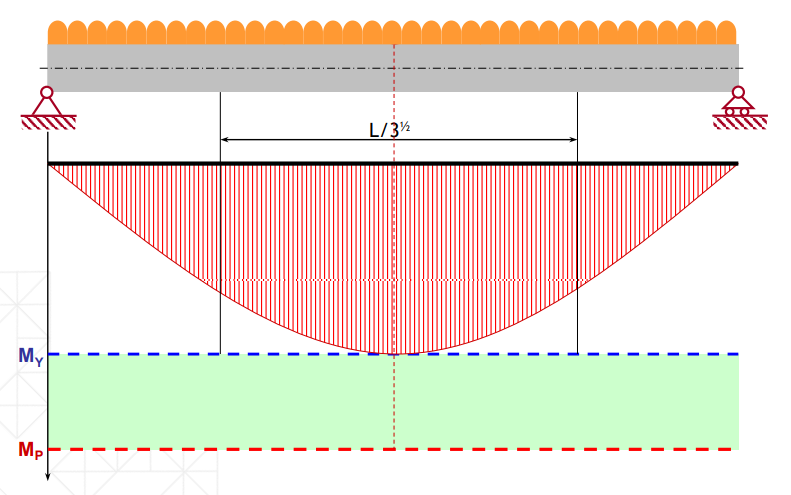
\includegraphics[width = 0.9 \textwidth]{../img/beam24.PNG}
  \caption{The moment increases as the load increases while keeping profile the same, reaching $M_Y$ at a certain point.}
\end{figure}
\begin{figure}[H]
  \centering
  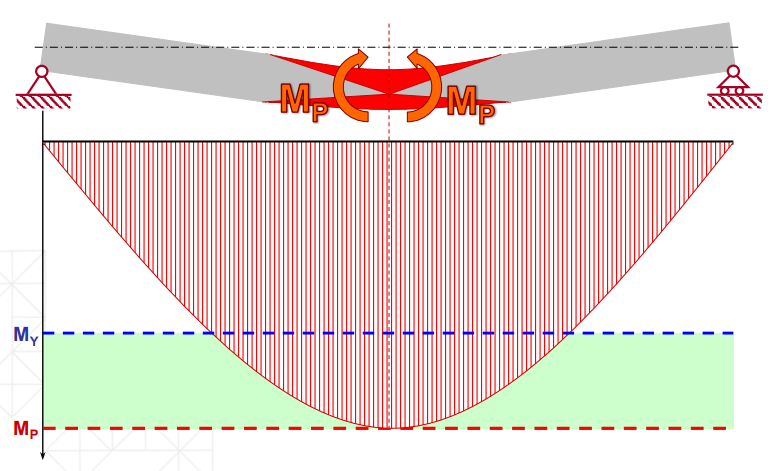
\includegraphics[width = 0.9 \textwidth]{../img/beam25.PNG}
  \caption{As the load is further increased, $M_P$ is reached. The spread of the plastic region occurs on both the cross-section and to the sides. Plastic hinge formations occurs.}
\end{figure}
\section{Collapse Mechanism}
In the following discussion we will also assume that: 
\begin{itemize}
  \item Cross sections behave elastically up to the plastic moment
  \item Plastic hinges affect only the section of maximum bending (partial yielding at points away from the plastic hinge is neglected)
  \item Failure modes other than plastic collapse are prevented
  \item Effect of normal and shear forces can be neglected
\end{itemize}
\subsection{Statically Determinate Beam}
\textbf{Collapse} occurs when a sufficient number of hinges have developed to reduce a structure to a mechanism. If the structure is \textbf{statically determinate} the development of a \textbf{single hinge} leads to collapse.
\subsubsection{\large Case 1: load factor for a beam with a concentrated central point load on a simple support}
\begin{figure}[H]
  \centering
  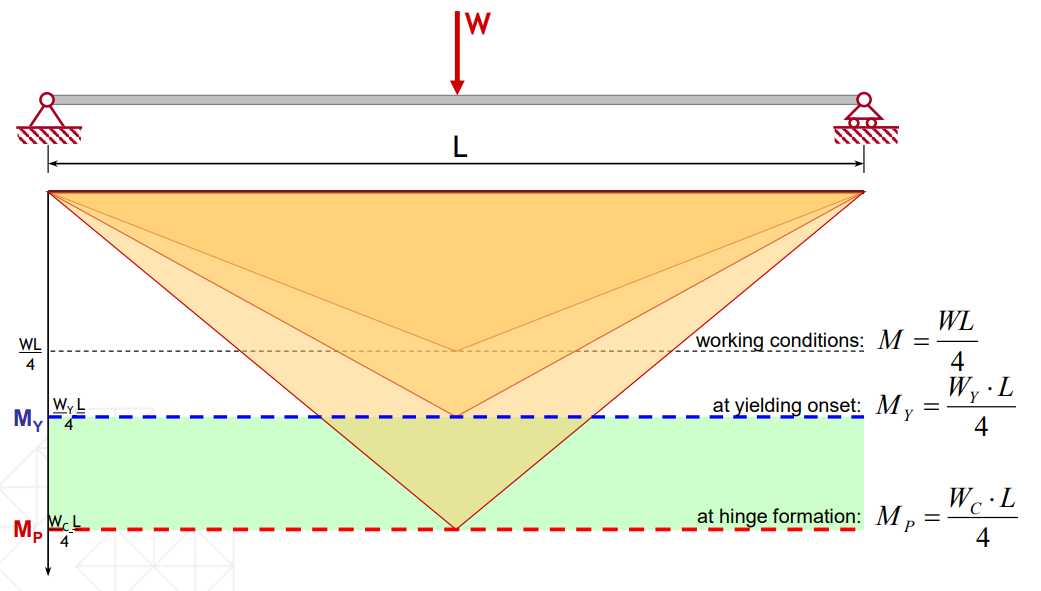
\includegraphics[width = 0.8 \textwidth]{../img/beam26.PNG}
  \caption{The beam under working condition, at yielding onset, and at hinge formation. The moment should be kept at/below the working condition for safety reasons.}
\end{figure}
The load that initiates yielding is:
\begin{gather}
  W_Y = \frac{4M_Y}{L}
\end{gather}
Collapse occurs at load:
\begin{gather}
  W_C = \frac{4M_P}{L}
\end{gather}
\subsubsection{\large Load Factor and Safety Factor}
The safety factor $K_S$, used when conventional elastic approach is adopted, is defined as the \textbf{ratio between the load that initiate yielding $W_Y$ and the maximum working load $W_{max}$}:
\begin{gather}
  K_S = \frac{W_Y}{W_{max}} \longrightarrow \text{This is what you decide}
\end{gather}
Similarly, the load factor $K_L$ is defined as the \textbf{ratio between the critical load $W_C$ that produces the structure’s collapse and the maximum working load $W_{max}$}:
\begin{gather}
  K_L = \frac{W_C}{W_{max}}
\end{gather}
For a statically determinate structure, the load factor $K_L$ corresponds to the product between the shape factor $f$ and the safety factor $K_S$: 
\begin{gather}
  K_L = f\cdot K_S
\end{gather}
In the case of statically indeterminate structures, more than one hinge is required, and therefore:
\begin{gather}
  K_L \geq f\cdot K_S
\end{gather}
\subsection{Statically Indeterminate Beam}
Collapse occurs when a sufficient number of hinges have developed to reduce a structure to a mechanism. If the structure is \textbf{statically determinate} the development of a \textbf{single hinge} leads to \textbf{collapse}. \\\\
If the structure is \textbf{statically indeterminate} the development of a \textbf{single hinge} leads to an \textbf{alternative structure, with higher degree of freedom}. In this case, before structure collapses, a sufficient number of hinges have to develop, in order to make the structure labile.
\subsubsection{\large Case 2: load factor for a propped cantilever with concentrated central load}
\begin{figure}[H]
  \centering
  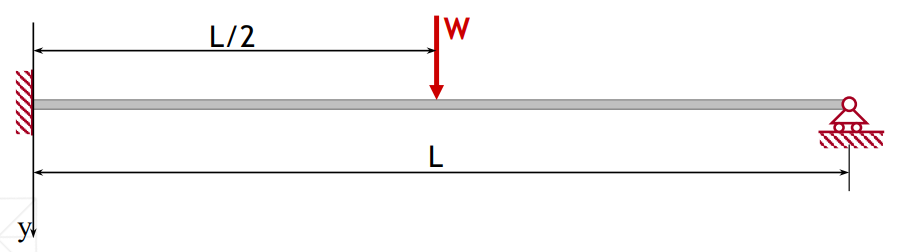
\includegraphics[width = 0.8 \textwidth]{../img/beam27.PNG}
\end{figure}
\begin{figure}[H]
  \centering
  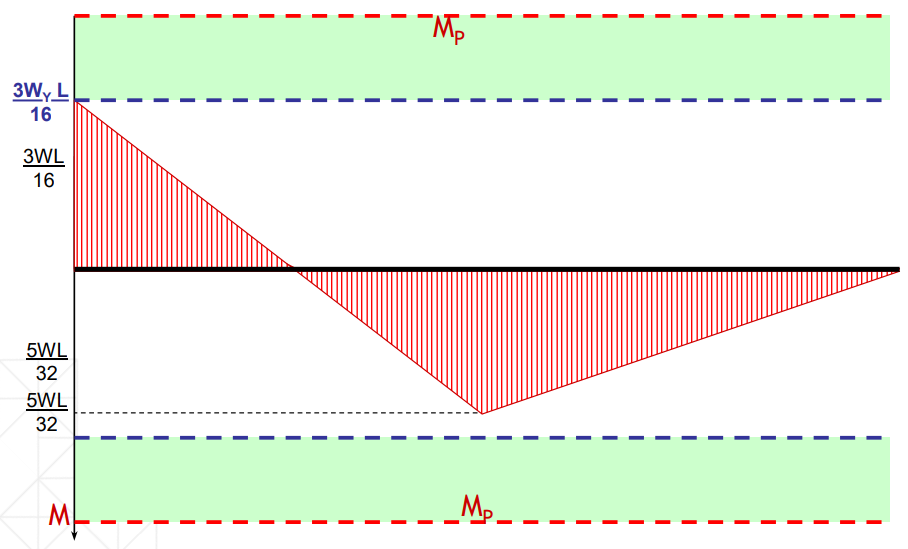
\includegraphics[width = 0.9 \textwidth]{../img/beam28.PNG}
  \caption{The moment diagrams when the load is increased to the yielding onset/moment}
\end{figure}
\begin{figure}[H]
  \centering
  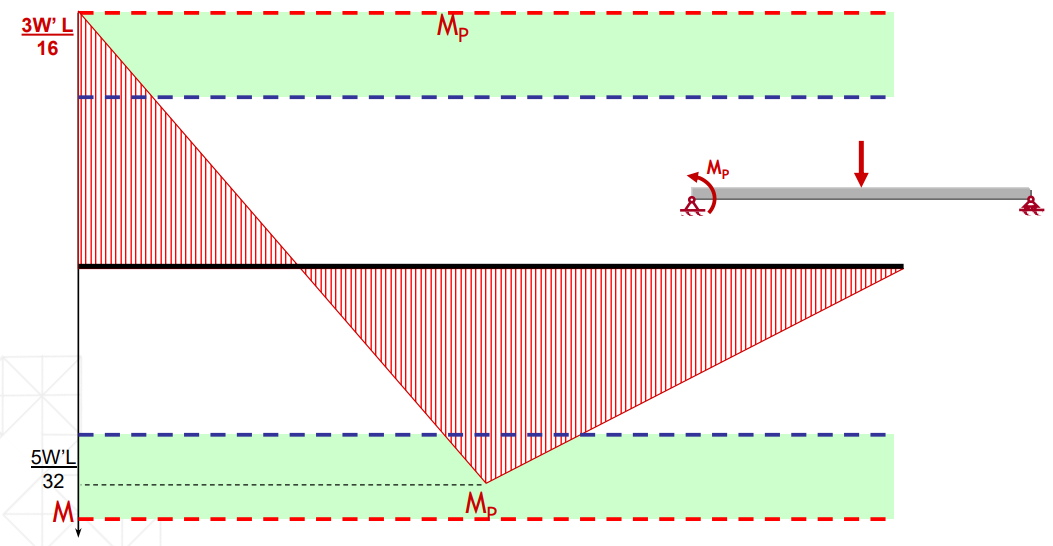
\includegraphics[width = 0.9 \textwidth]{../img/beam29.PNG}
  \caption{The moment diagrams when the highest moment (on the left) reaches plastic moment, and the moment at the midpoint surpasses the yielding moment. At this point, a plastic hinge is formed at the left end of this beam, hence the boundary condition changes. However, the plastic moment $M_P$ to resist the bending still exists.}
\end{figure}
\begin{figure}[H]
  \centering
  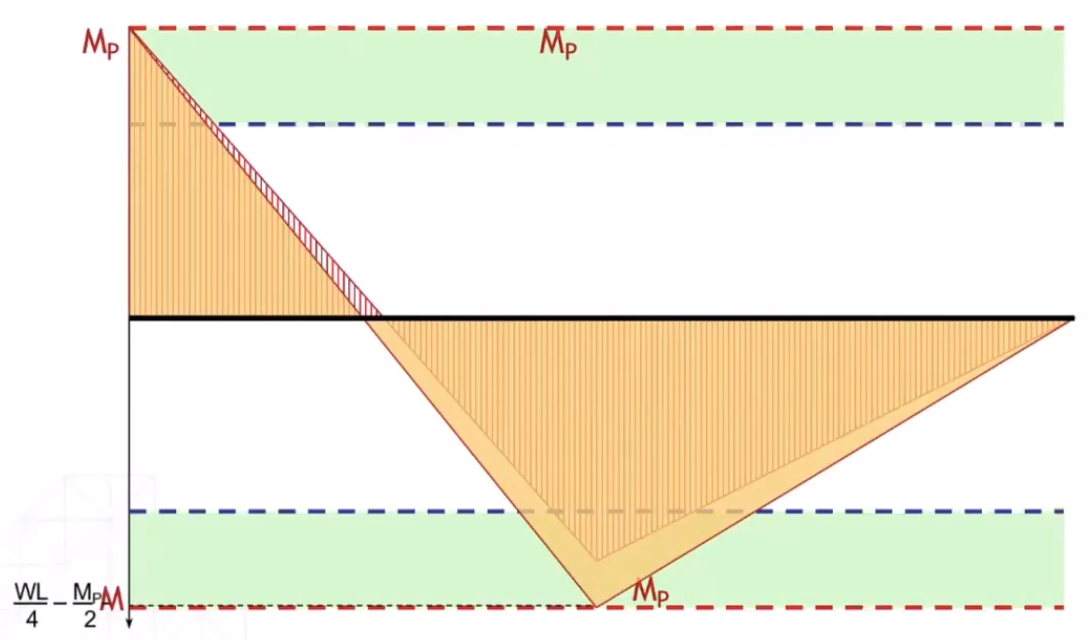
\includegraphics[width = 0.9 \textwidth]{../img/beam30.PNG}
  \caption{The additional load $W''$ will further increase the bending moment at the midspan, that will eventually reach the plastic moment and form another hinge: the structure will become labile and collapse.}
\end{figure}
The load that initiates yielding is:
\begin{gather}
  W_Y = \frac{16M_Y}{3L}
\end{gather}
First hinges formation occurs at load:
\begin{gather}
  W' = \frac{16M_P}{3L}
\end{gather}
Collapse occurs at load:
\begin{gather}
  W_C = \frac{6M_P}{L}
\end{gather}
The Load Factor is:
\begin{gather}
  K_L = \frac{9}{8}f\cdot K_S \\[5pt]
  K_L = \frac{W_C}{W_Y}K_S = \frac{6M_P/L}{16M_Y/3L}K_S = \frac{9}{8}f\cdot K_S
\end{gather}
Where:
\begin{itemize}
  \item $\frac{9}{8}$ depends on the beam cross section
  \item $f$ depends on loading and boundary conditions
\end{itemize}
\subsubsection{\large Load Deflection Curve}
\begin{figure}[H]
  \centering
  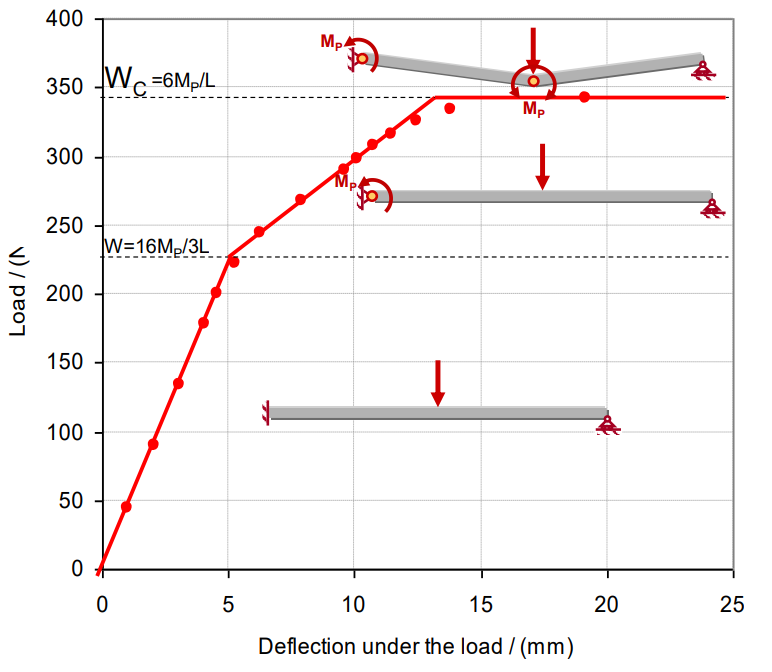
\includegraphics[width = 0.8 \textwidth]{../img/graph8.PNG}
  \caption{Experimental Load-Deflection Characteristic}
\end{figure}
\end{document}